% main.tex --- Measuring Complex Tastes
% Tables and figures are generated by scripts/01--03; do not edit numbers by hand.
\documentclass[12pt]{article}

\usepackage[margin=1in]{geometry}
\usepackage{graphicx}
\usepackage{booktabs}
\usepackage{amsmath}
\usepackage{caption}
\usepackage[round]{natbib}
\usepackage[colorlinks=true,linkcolor=blue,citecolor=blue,urlcolor=blue]{hyperref}
\usepackage{dcolumn}

\graphicspath{{figures/}}

\title{Measuring Complex Tastes: A Multiple Factor Analysis of Preferences, Consumption, and Evaluations in Musical Taste}

\author{Omar Lizardo\\ \small University of California, Los Angeles} \date{October 2026}

\begin{document}

\maketitle

\begin{abstract}
\noindent This paper proposes an approach to measuring complex tastes in data that include preferences, engagement, and evaluations of the same set of objects, whether genre categories or specific cultural objects. I take a Geometric Data Analysis (GDA) approach based on Multiple Factor Analysis (MFA). The method lets us answer concrete substantive questions about complex tastes, including whether preferences, engagement, and evaluations are equally potent determinants of complex tastes, and whether some complex taste dimensions relate more or less to others. In addition, the method captures the duality of complex tastes: individuals are more or less likely to be sources of complex tastes (some individuals have simple tastes, others more complex ones), and genres/objects are more or less likely to be targets (with some genres being more likely to have simple versus complex taste profiles). I demonstrate the approach's utility using data on Americans' complex tastes for twenty musical genres collected circa 2012.
\end{abstract}

\section{Introduction}

Sociologists measure cultural taste in at least three distinct ways \citep{ma2026tastes}. One tradition takes taste to be a \emph{preference}---a person's affective response toward a cultural object. A second takes taste to be an orientation toward \emph{consumption}---realized participation or engagement within a cultural field. A third takes taste to be a faculty expressed in \emph{valuations}---judgments about the quality or status of cultural objects. Rather than treating this semantic ambiguity as a defect to be resolved by fiat, \citet{ma2026tastes} argues that taste should be conceptualized pluralistically as a person's ``thick subjectivity'' in a cultural field: a multidimensional orientation expressed through multiple aspects of action that guides our preferences, engagement, and evaluations.

Recognizing that taste has multiple aspects sharpens the formulation of \emph{complex taste} phenomena. Simple tastes are those in which the aspects are harmonized: what a person likes, what they consume, and what they value point in the same direction. Complex tastes, by contrast, are configurations in which the aspects disagree---the guilty pleasure (liked and consumed but disvalued), the taste pose (liked and valued but not consumed), distanced consumption (consumed but neither liked nor valued), and their kin \citep{ma2026tastes}. Complex tastes, on this view, cannot be described by recourse to any single mode of action.

This paper develops a measurement strategy for complex tastes that takes the pluralist conception seriously. The strategy uses Multiple Factor Analysis (MFA) \citep{pages2014mfa,abdi2013mfa}, a member of the Geometric Data Analysis (GDA) family used by  \citet{bourdieu1984distinction} in his classic study \citep{rouanet2000geometric-a44, roux2004geometric-65c}, applied to a data structure in which each cultural object is described by three sets of indicators, one for each aspect of taste. The block structure of the MFA allows us to ask the questions the theory makes salient: how strong are the links between preference, consumption, and evaluation? Do the aspects contribute equally to the shared structure of taste? And where, geometrically, do complex tastes live?

\section{Data and Measures}

\subsection{Data}

I use the Survey Sample International (SSI) 2012 Cultural Tastes Survey \citep{lizardo2012ssi}, a national sample of $N = 2{,}276$ American adults collected circa 2012. The survey contains, for each of twenty musical genres, measures of the respondent's liking of the genre, their consumption of the genre, and their perceptions of the social characteristics of the genre's typical fans. After listwise deletion of the $17$ cases with missing data on any of the $60$ analysis variables, the analytic sample contains $N = 2{,}259$ valid respondents.

\subsection{Measures: Three Aspects of Taste for Twenty Genres}

Each genre contributes three binary indicators, one per aspect, yielding $20 \times 3 = 60$ variables organized into three blocks of twenty.

\begin{description}
\item[Preference (liking).] Respondents rated how much they like each genre on a four-point scale (like; dislike; neither like nor dislike; not familiar). A genre is coded $1$ if the respondent likes it and $0$ otherwise; unfamiliarity is treated as non-liking, consistent with the reading that an affective response requires familiarity with the object.
\item[Consumption (engagement).] Respondents checked which of the twenty genres they had listened to in the past month ($1 = $ listened, $0 = $ otherwise).
\item[Evaluation (status valuation).] Respondents indicated, from a list of social characteristics, the attributes of the genre's \emph{typical fan}. These items are check-all-that-apply, so the categories are not mutually exclusive: a respondent may indicate both that the typical fan is a college graduate and that they did not attend college, or that they are both working and upper class. A genre is coded $1$ if the respondent attributed \emph{unambiguously} high status to its typical fans---that is, if they indicated that the typical fan is a college graduate without also indicating no college, \emph{or} middle or upper class without also indicating working or lower class---and $0$ otherwise.
\end{description}

Table~\ref{tab:genre-rates} reports the proportion of respondents coded $1$ on each indicator. Overall, $41.7\%$ of genre-responses are positive on the preference measure, $22.9\%$ on consumption, and $20.7\%$ on evaluation. The unambiguous-status standard is demanding---it requires an uncontested high-status signal in at least one domain---and evaluation is accordingly the least frequently affirmed aspect: respondents grant unambiguous high status to a genre's fans less readily than they like the genre or have recently listened to it.

\begin{table}[htbp]
\centering \caption{Proportion of respondents coded 1 on each aspect indicator, by genre ($N = 2{,}259$).}
\label{tab:genre-rates}
\begin{tabular}{lccc}
\toprule
Genre & Preference & Consumption & Evaluation \\
\midrule
Classical & 55.1 & 31.8 & 53.4 \\
Opera & 20.0 & 8.5 & 52.1 \\
Jazz & 50.9 & 24.1 & 35.5 \\
Broadway/Show & 42.8 & 16.9 & 44.1 \\
Mood/Easy & 57.8 & 31.0 & 35.6 \\
Big Band & 39.0 & 12.7 & 28.2 \\
Classic Rock/Oldies & 73.1 & 48.3 & 34.4 \\
Country & 48.7 & 40.1 & 25.4 \\
Bluegrass & 28.8 & 8.2 & 15.3 \\
Folk & 28.2 & 9.4 & 22.0 \\
Hymns/Gospel & 38.2 & 21.0 & 30.3 \\
Latin/Spanish/Salsa & 29.0 & 17.1 & 25.1 \\
Rap/Hip-Hop & 31.1 & 28.7 & 18.4 \\
Blues/R\&B & 53.0 & 27.1 & 29.4 \\
Reggae & 32.5 & 13.3 & 19.1 \\
Top 40/Pop & 56.8 & 39.5 & 34.9 \\
Contemporary Rock & 51.0 & 26.8 & 30.8 \\
Indie/Alt Rock & 30.5 & 16.9 & 23.5 \\
Dance/Club & 43.0 & 21.2 & 30.9 \\
Heavy Metal & 24.9 & 15.8 & 17.8 \\
\midrule
Overall & 41.7 & 22.9 & 30.3 \\
\bottomrule
\end{tabular}

\end{table}

\section{Analytic Strategy}

Multiple Factor Analysis \citep{pages2014mfa,abdi2013mfa} is designed for data structures of this kind: a set of individuals described by several blocks of variables measured on the same individuals, with the goal of a common representation that treats the blocks---here the three aspects of complex tastes---as comparable without letting any one block dominate ex ante.\footnote{The MFA literature calls these sets of variables ``groups'' \citep{pages2014mfa}. We speak of \emph{blocks of variables}---or of \emph{aspects}, when referring to the three blocks of this application---reserving ``group'' for its ordinary sociological meaning. In the geometric data analysis tradition from which MCA derives, the distinct values that a categorical variable can take---here \emph{yes} and \emph{no}---are called its \emph{modalities} \citep{rouanet2000geometric-a44}; we call them \emph{categories} throughout.} Throughout, we use \emph{aspect} for one of the three ways of measuring taste distinguished in the introduction---preference, engagement, and evaluation---each entering the analysis as its own block of twenty genre indicators. Here we analyze a table with as many rows as individuals in the data and sixty columns that designate each individual's preferences, consumption, and evaluation of twenty musical genres. The $ij^{th}$ cell in the data, corresponding to row $i$ and column $j$, equals one if individual $i$ likes, consumes, or evaluates genre $j$ highly.

MFA proceeds in two steps. First, we analyze each block of variables separately by running a separate Multiple Correspondence Analysis (MCA) on each of the three individual-by-genre tables (20 columns and the same number of individuals), one table per aspect (preference, consumption, and evaluation).\footnote{A robustness check verifies that the choice of MCA as the GDA analytic engine is not driving the results: re-estimating the same MFA with each block analyzed instead by a scaled PCA of the binary indicators leaves the substantive results intact. The eigenvalues agree to two decimals ($1.504$, $1.188$, and $0.997$ versus $1.509$, $1.178$, and $0.982$ on the first three dimensions); the RV structure is unchanged (preference--consumption $0.32$; evaluation--preference and evaluation--consumption $0.01$ and $0.01$); individual coordinates correlate at $0.98$, $0.97$, and $0.84$ across the first three dimensions (up to sign), and the complex-taste scores at $0.96$, $0.89$, and $0.77$; the antinomy shares of projected partial inertia are $56\%$, $53\%$, and $61\%$, against $56\%$, $52\%$, and $63\%$ in the MCA version. The one substantive difference concerns rare categories: MCA gives them proportionally more weight, stretching the most distinctive affirmations---here a feature, since the rare affirmations carry the theoretical interest.} Second, we combine the separate analyses into a global analysis, weighting each block by the inverse of the first eigenvalue of its separate analysis to ensure that all three aspects contribute comparably to the global structure, regardless of the strength of the first dimension. Here, the global structure is the ``complex taste space,'' and each separate space is the space of one aspect of complex taste (preference, engagement, and evaluation).

The MFA approach provides quantities that, in turn, answer the measurement questions posed by the study of complex tastes. The first question is whether the three aspects are redundant or partially independent; the latter is required to justify studying complex tastes in the first place. After all, if preferences contained the same information as either consumption or evaluation, then studying simple tastes based on preferences would be sufficient. The \textit{RV coefficient} between two blocks of variables (here, complex-taste aspects) is a global measure of the similarities of the geometries that two blocks impose on the same individuals---the multivariate analog of a squared correlation between two block-specific images of the respondents, running from 0 (nothing in common) to 1 (the same structure).\footnote{For each block $h$, let $\mathbf{S}_h$ be the block's configuration matrix: the matrix of weighted cross-products between respondents induced by its twenty indicators, $\mathbf{S}_h = \mathbf{Z}_h \mathbf{W}_h \mathbf{Z}_h'$, where $\mathbf{Z}_h$ is the centered indicator matrix and $\mathbf{W}_h$ holds the MCA column weights. The $(i,i')$ entry of $\mathbf{S}_h$ is large when respondents $i$ and $i'$ answer alike on that aspect's twenty genres. The RV coefficient between blocks $h$ and $k$ is $\mathrm{RV}(h,k) = \mathrm{tr}(\mathbf{S}_h \mathbf{S}_k) / \sqrt{\mathrm{tr}(\mathbf{S}_h^2)\,\mathrm{tr}(\mathbf{S}_k^2)}$: the cosine between the two configurations viewed as vectors of pairwise respondent similarities.} If preference, engagement, and evaluation induced similar structures, any one of them could stand in for the others, and a person's tastes could be measured as simple tastes. Small RV coefficients mean instead that each aspect carries information the others lack: they establish, at the level of the data structure, the possibility of complex tastes---respondents whose aspects do not line up---before any individual is measured.

The second question is whether each aspect actually participates in the common representation that the MFA builds from them. The \textit{$Lg$ coefficient} measures the strength of the link between a block of variables and the global structure: how much of the block's own geometry is expressed in the global space.\footnote{Formally, $Lg(h,k) = \mathrm{tr}(\mathbf{S}_h \mathbf{S}_k) / \sqrt{\mathrm{tr}(\mathbf{S}_h^2)}$: the numerator of the RV coefficient, normalized by the first block's inertia alone. Because the link is not divided by the second structure's overall strength, $Lg$ measures the association on an absolute scale, and $Lg(h,k) \neq Lg(k,h)$. $Lg(h, \mathrm{MFA})$ takes the compromise configuration $\mathbf{S}_{\mathrm{MFA}}$ as the second argument.} The $Lg$ coefficient assigns a single number to each aspect---it asks about the aspect's participation in the compromise as a whole, not about any one dimension of it---and because it is measured on an absolute scale it can be compared across aspects and against the common structure. The balancing weights ensure equal influence for the three aspects at the outset, not equal presence in the result; an aspect with a much weaker internal structure could, in principle, be present in name only. The $Lg$ coefficients therefore tell us whether each of the three aspects of complex taste leaves a detectable imprint on the complex taste space, or whether the compromise quietly drops one of them.

The third question is different: not how the aspects relate to one another or to the compromise, but which aspect organizes each dimension of the shared space. The \textit{aspect contributions}---called \emph{group contributions} in the MFA literature---apportion each dimension of the common representation among the three aspects---the share of the dimension's variance carried by each aspect.\footnote{Formally, the contribution of aspect $h$ to dimension $s$ is $\mathrm{ctr}(h,s) = \sum_{j \in h} w_j f_{js}^2 / \lambda_s$: the sum over the aspect's twenty variables of their weighted squared coordinates on the dimension, divided by the dimension's eigenvalue $\lambda_s$; the three aspects' contributions sum to $100\%$ on every dimension.} Note that this is different from what the $Lg$ coefficient tells us. While the $Lg$ coefficients assign each aspect one number, the aspect contributions assign each dimension one decomposition across aspects. The contributions reveal whether the axes of the taste space are jointly constituted by preference, engagement, and evaluation or are, in substance, the axis of one aspect echoed in the others---whether one dimension is dominated by consumption at the expense of preference and evaluation, or is equitably defined by all three. This matters for complex tastes because a dimension dominated by a single aspect---one organized by what respondents praise rather than by what they prefer or consume---is precisely where the aspects can come apart, and therefore where complex tastes should appear. 

The MFA's block structure also provides the machinery to measure complex tastes directly in the geometry of the space. In the combined representation, each individual $i$ is associated with $H$ \emph{partial points}---one per aspect, so $H = 3$ here---whose average is the individual's global point. For a given dimension $s$, the projected partial inertia of individual $i$ decomposes exactly as
\begin{equation}
\sum_{h=1}^{H} F_{sh}(i)^2 \;=\; H \cdot F_s(i)^2 \;+\;
\underbrace{\sum_{h=1}^{H} \left(F_{sh}(i) - F_s(i)\right)^2}_{W_s(i)},
\label{eq:decomp}
\end{equation}
where $H$ is the number of aspects (three here), $h = 1, \dots, H$ indexes them, $F_s(i)$ is the individual's global coordinate, and $F_{sh}(i)$ their partial coordinate from aspect $h$. The first term locates the individual in the common space; the second, $W_s(i)$, measures how dispersed the aspect-specific points are around that common position. It is zero when the three aspects place the individual identically---the geometry of a simple taste---and grows with disagreement between aspects. We therefore call $W_s(i)$ the individual's \emph{complex-taste score} on dimension $s$. The squared pairwise distances between partial points ($d^2_{s,\text{pref-cons}}(i)$, $d^2_{s,\text{pref-eval}}(i)$, $d^2_{s,\text{cons-eval}}(i)$)\footnote{On dimension $s$, the squared distance between the partial points of aspects $h$ and $k$ is the squared difference of their coordinates on that dimension, $d^2_s(h,k) = \left(F_{sh}(i) - F_{sk}(i)\right)^2$. The three pairwise distances sum exactly to $H$ times the complex-taste score, $\sum_{h<k} d^2_s(h,k) = H \cdot W_s(i)$, in consequence of the identity $\sum_{h<k}\left(F_{sh}(i) - F_{sk}(i)\right)^2 = H \sum_{h=1}^{H} F_{sh}(i)^2 - \left(\sum_{h=1}^{H} F_{sh}(i)\right)^2$ together with $F_s(i) = H^{-1} \sum_{h=1}^{H} F_{sh}(i)$.} further decompose $W_s(i)$ into disagreement between specific pairs of aspects: the three distances sum to $H \cdot W_s(i)$, and each pair's share of that sum isolates the disagreement for which that pair of aspects is responsible.\footnote{As the discrete complement to this geometric measure, each genre--respondent pair is classified into one of Ma's eight configurations from the binary triple of orientations (preference, consumption, evaluation): the simple taste $(+++)$, the simple non-taste $(---)$, and the six complex tastes (Appendix~\ref{app:configurations}).}

The decomposition is easiest to grasp with an example (Figure~\ref{fig:worked-example}). Consider a respondent who likes fifteen of the twenty genres---from jazz, Broadway/show tunes, and classic rock/oldies to top 40 and contemporary rock---listens to nine of them, and credits the fans of eighteen genres with unambiguously high status. On the first (horizontal) dimension, the general-affirmation axis, all three aspect points sit on the same side of the origin---preference at $+3.53$, consumption at $+3.05$, evaluation at $+2.28$, around a global point of $+2.95$---so the aspects disagree only about \emph{how much} this respondent engages, and only modestly: $W_1 = 0.8$, or 3\% of the projected partial inertia. The third (vertical) dimension, the status-valuation axis, tells a different story. The preference and consumption points sit slightly on the withholding side of the origin ($-0.66$ and $-1.33$), while the evaluation point lies far out on the side anchored by the genre evaluations ($+13.12$): the respondent grants high status to nearly every genre's fans, a generosity of valuation that far outruns both their liking and their listening. The global point is $+3.71$, and the disagreement now dwarfs the position: $W_3 = (-0.66 - 3.71)^2 + (-1.33 - 3.71)^2 + (13.12 - 3.71)^2 = 133.1$, or 76\% of the projected partial inertia---nearly everything that places this respondent on the status-valuation dimension is disagreement between aspects rather than shared orientation.\footnote{In Ma's combinatorial terms (see Appendix~\ref{app:configurations}), the same respondent holds thirteen genres in complex configurations: one guilty pleasure, seven taste poses, four instances of distant praise, and one instance of distanced consumption.} The second dimension completes the illustration in a different register (right panel of Figure~\ref{fig:worked-example}): the preference point sits just on the popular side of the origin ($-0.89$), while consumption and evaluation sit on the highbrow side ($+1.74$ and $+4.31$), around a global point of $+1.72$, so that $W_2 = 13.5$---60\% of the projected partial inertia. A single summary number would miss this structure: the same respondent carries a small $W_1$ and an extreme $W_3$, which is why the complex-taste scores are reported dimension by dimension.

\begin{figure}[htbp]
\centering
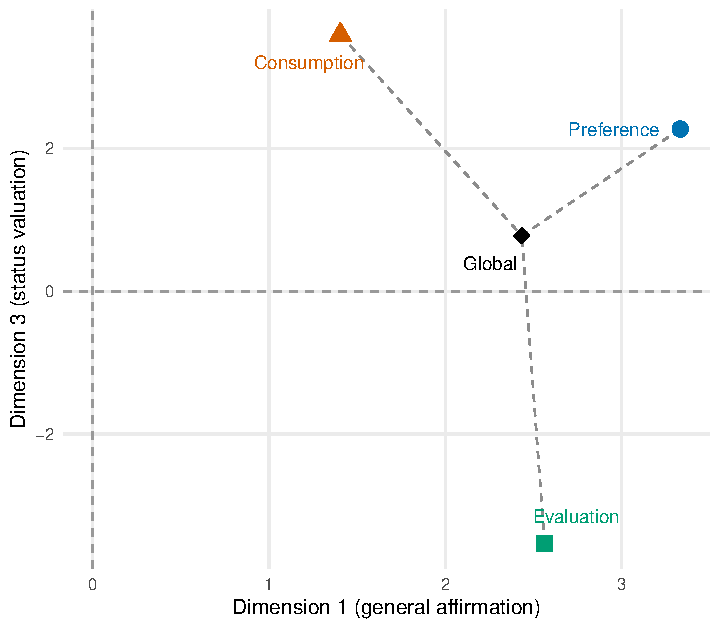
\includegraphics[width=.9\linewidth]{fig-worked-example} \caption{Worked example: partial points of one respondent, shown against the status-valuation axis (Dimension 3). The left panel pairs it with the general-affirmation axis (Dimension 1), the right panel with the highbrow--popular axis (Dimension 2). Colored points are the aspect-specific partial points; the black diamond is the respondent's global (compromise) position, their average. Dashed segments connect each partial point to the compromise. In the left panel, the sum of squared horizontal deviations from the compromise is $W_1 = 0.8$ (3\% of the projected partial inertia) and the sum of squared vertical deviations is $W_3 = 133.1$ (76\%); in the right panel, the horizontal deviations give $W_2 = 13.5$ (60\%).}
\label{fig:worked-example}
\end{figure}

The analysis was conducted in \textsf{R} with \textsf{FactoMineR}; scripts reproducing all results are available with the replication materials.

\section{Results}

\subsection{Overall Structure of the Taste Space}

Table~\ref{tab:eigen} reports the eigenvalue decomposition. The first dimension ($\lambda_1 = 1.51$) accounts for $9.6\%$ of the variance and the second ($\lambda_2 = 1.18$) for $7.5\%$; the first five dimensions cumulate to $32.5\%$. Percentages of this magnitude are typical for categorical GDA of sparse binary indicators, where a large share of the variance is idiosyncratic genre-by-genre variation.

\begin{table}[htbp]
\centering \caption{Eigenvalues of the MFA (first five dimensions).}
\label{tab:eigen}
\begin{tabular}{lccc}
\toprule
Dimension & Eigenvalue & \% variance & Cumulative \% \\
\midrule
$1$ & 1.667 & 12.3 & 12.3 \\
$2$ & 1.193 & 8.8 & 21.1 \\
$3$ & 0.899 & 6.6 & 27.8 \\
$4$ & 0.715 & 5.3 & 33.1 \\
$5$ & 0.648 & 4.8 & 37.9 \\
\bottomrule
\end{tabular}

\end{table}

\begin{figure}[htbp]
\centering
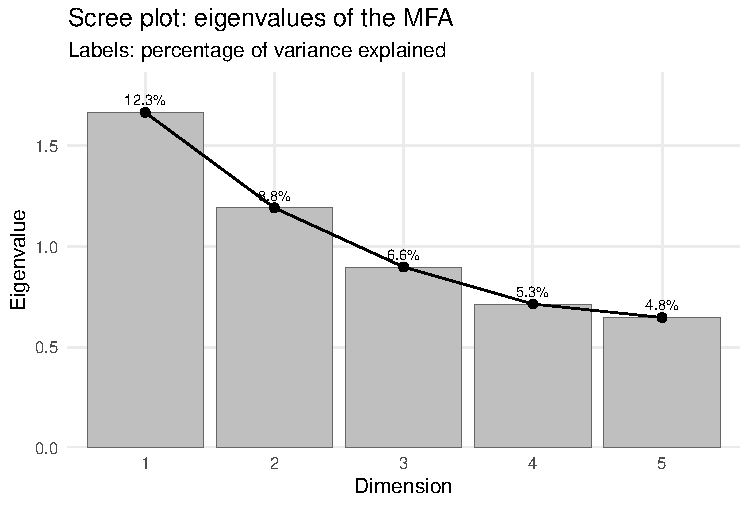
\includegraphics[width=.75\linewidth]{fig-scree} \caption{Scree plot of the MFA. Labels give the percentage of variance explained by each dimension.}
\label{fig:scree}
\end{figure}

The category coordinates support a reading of the first two dimensions. On the first dimension, the ``yes'' categories of preference and consumption are arrayed on the positive side of the origin---listening to folk ($+1.43$), bluegrass ($+1.34$), reggae ($+1.24$), and opera ($+1.13$) are the most extreme (for their rarity) consumption affirmations---while the corresponding ``no'' categories occupy the negative side. The genre evaluations, by contrast, barely differentiate respondents on this axis: attributing unambiguous high status to a genre's fans ranges only from $+0.03$ (Broadway/show tunes) to $+0.53$ (rap/hip-hop), an order of magnitude less distinctive than the consumption affirmations. Dimension 1 is thus a \emph{general affirmation} axis: a gradient in the overall propensity to like and to listen, ordering respondents from generalized non-engagement to generalized engagement with the genre system. Affirming the rarest categories receives the most extreme scores, as is typical of MCA \citep{rouanet2000geometric-a44}; the status attributions concentrate their distinctiveness on the third dimension, to which we return below.

The second dimension, shown in the category map (Figure~\ref{fig:categories}), organizes genres hierarchically rather than by aspect. At one pole sit the ``yes'' categories of the consecrated, highbrow end of the genre system (big band $+0.98$, opera $+0.86$, Broadway and show tunes $+0.84$, classical and bluegrass $+0.73$, folk $+0.68$); at the other pole sit rap/hip-hop ($-0.91$ and $-0.84$ for consumption and preference), indie and alternative rock ($-0.84$), heavy metal ($-0.78$), dance/club ($-0.75$), and reggae ($-0.63$). Dimension 2 is therefore a \emph{highbrow--popular} axis that holds within each of the three aspects simultaneously---the same opposition that classical work in the field has located at the core of musical taste structures \citep{bourdieu1984distinction}. The individual factor maps (Figure~\ref{fig:individuals}) preview this axis's social anchoring: respondents' positions are strongly ordered by age, with the youngest cohort sitting toward the popular pole and the oldest toward the highbrow pole (Section~\ref{sec:social}). The map's vertical axis also offers a first look at Dimension 3: all twenty ``yes'' categories of the genre evaluations sit on one side of the origin---the visible signature of a distinct \emph{status-valuation} axis, opposing the evaluation aspect to both the preference and consumption aspects.

\begin{figure}[htbp]
\centering
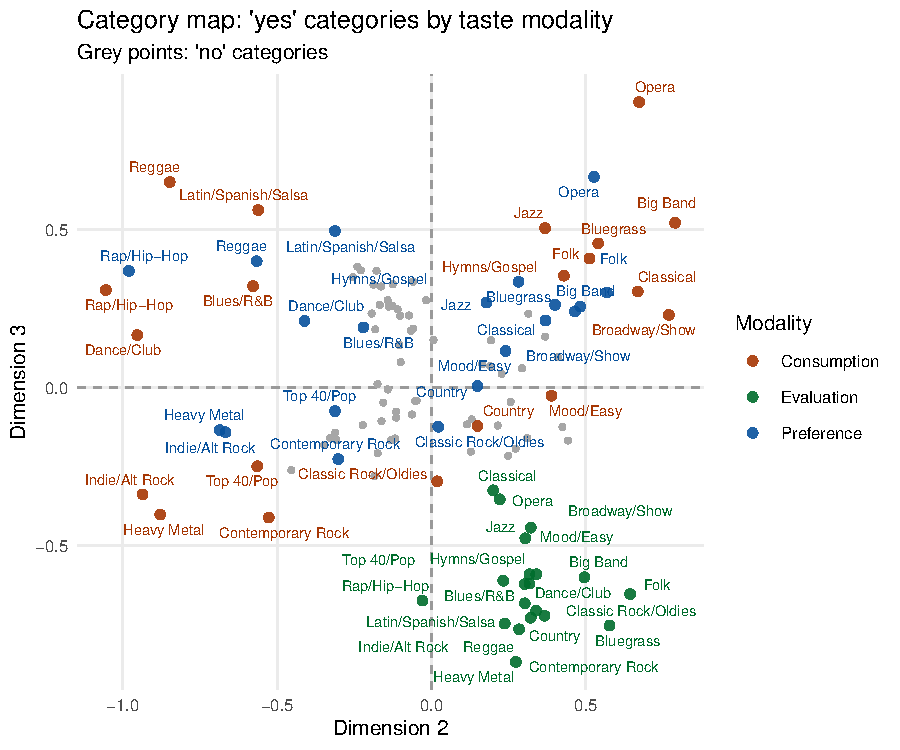
\includegraphics[width=.85\linewidth]{fig-categories} \caption{Category map of the MFA (dimensions 2--3). Colored points are the ``yes'' categories of each aspect; grey points are the corresponding ``no'' categories.}
\label{fig:categories}
\end{figure}

\begin{figure}[htbp]
\centering
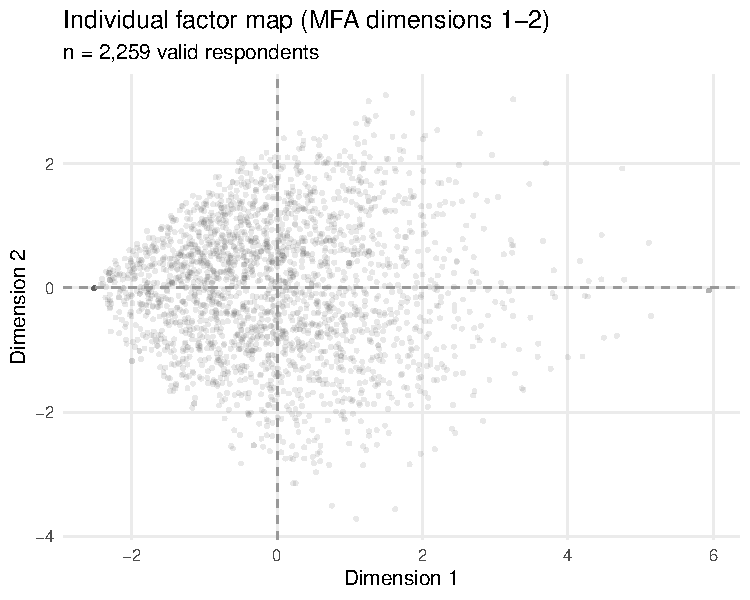
\includegraphics[width=.8\linewidth]{fig-individuals} \caption{Individual factor map (dimensions 2--3), points colored by age group; darker shades indicate older age groups. Each point is a respondent.}
\label{fig:individuals}
\end{figure}

\subsection{The Aspect Structure: How Independent Are Preference, Engagement, and Evaluation?}

The central result bears on the first question posed above: whether the three aspects are redundant or partially independent. The RV coefficients (Table~\ref{tab:rv}) answer it in favor of partial independence. The preference and consumption aspects are moderately linked ($RV = 0.32$): those who like a genre are somewhat more likely to have listened to it, but the two structures are far from interchangeable. By contrast, the evaluation aspect is nearly orthogonal to both ($RV = 0.01$ with each).

\begin{table}[htbp]
\centering \caption{RV coefficients between the three aspects and the MFA.}
\label{tab:rv}
\begin{tabular}{lcccc}
\toprule
 & Preference & Consumption & Evaluation & MFA \\
\midrule
Preference & 1.000 & 0.321 & 0.049 & 0.724 \\
Consumption & 0.321 & 1.000 & 0.060 & 0.788 \\
Evaluation & 0.049 & 0.060 & 1.000 & 0.426 \\
MFA & 0.724 & 0.788 & 0.426 & 1.000 \\
\bottomrule
\end{tabular}

\end{table}

This near-orthogonality is the geometric signature of the complex taste idea. Status attributions about who listens to a genre form a structurally independent aspect of taste that people's likes and actions cannot recover. A respondent's evaluation profile is, to a first approximation, empirically distinct from their preference and consumption profiles. Complex tastes---configurations in which the aspects disagree---are therefore not measurement noise or respondent inconsistency; they are the expected product of applying three weakly coupled measurement systems to the same objects.

\subsection{Which Aspects Drive Which Dimensions?}
\label{sec:contrib}

Table~\ref{tab:groups} reports the quantities that answer the second and third questions posed above: whether each aspect actually participates in the compromise the MFA builds from them, and which aspect organizes each dimension of the shared space. MFA's balancing weights---the inverses of the first eigenvalues of the separate analyses ($5.00$ for preference, $6.45$ for consumption, and $4.28$ for evaluation)---put the three aspects on equal footing; the separate analyses' first eigenvalues are of comparable strength ($0.20$, $0.16$, and $0.23$).

\begin{table}[htbp]
\centering \caption{First eigenvalues and balancing weights of the separate analyses, aspect contributions to the first three dimensions, and $Lg$ coefficient with the MFA.}
\label{tab:groups}
\begin{tabular}{lcccccc}
\toprule
 & & & \multicolumn{3}{c}{Contributions (\%)} & \\
\cmidrule(lr){4-6}
Aspect & $\lambda_1$ & Weight ($1/\lambda_1$) & Dim 1 & Dim 2 & Dim 3 & $Lg$ with MFA \\
\midrule
Preference & 0.200 & 5.004 & 48.1 & 40.0 & 8.0 & 1.95 \\
Consumption & 0.155 & 6.452 & 49.4 & 48.9 & 8.1 & 2.48 \\
Evaluation & 0.234 & 4.277 & 2.5 & 11.0 & 83.9 & 1.14 \\
\bottomrule
\end{tabular}

\end{table}

\begin{table}[htbp]
\centering \caption{Partial axes: correlations between each aspect's separate-analysis axes and the first three MFA dimensions.}
\label{tab:partial-axes}
\begin{tabular}{lccc}
\toprule
Partial axis & Dim 1 & Dim 2 & Dim 3 \\
\midrule
Preference axis 1 & 0.84 & 0.13 & -0.16 \\
Preference axis 2 & 0.17 & -0.87 & 0.25 \\
Preference axis 3 & 0.04 & -0.04 & -0.14 \\
\addlinespace
Consumption axis 1 & 0.86 & -0.11 & -0.07 \\
Consumption axis 2 & 0.01 & 0.89 & -0.28 \\
Consumption axis 3 & 0.03 & -0.03 & -0.11 \\
\addlinespace
Evaluation axis 1 & 0.19 & 0.35 & 0.91 \\
Evaluation axis 2 & 0.01 & -0.06 & -0.02 \\
Evaluation axis 3 & -0.08 & -0.03 & 0.02 \\
\bottomrule
\end{tabular}

\end{table}

On the third question, the answer is that the dimensions are not aspect-neutral. Preference and consumption jointly organize the first two dimensions (contributing $48.1\%$ and $49.4\%$ to Dimension 1, and $40.0\%$ and $48.9\%$ to Dimension 2). The third dimension is different in kind: evaluation contributes $83.9\%$, against $8.0\%$ and $8.1\%$ for the other two aspects. The content of the dimension is unambiguous: \emph{every one} of the twenty evaluation ``yes'' categories lies on the same (positive) side of Dimension 3 (mean coordinate $+1.12$; range $+0.20$ to $+1.87$), while the ``yes'' categories of preference and consumption collapse toward the origin on it (ranges $-0.41$ to $+0.12$ and $-0.59$ to $+0.21$). The evaluation categories are themselves ordered by rarity: granting high status to the fans of rap/hip-hop ($+1.87$), Latin/Spanish/Salsa ($+1.84$), or country ($+1.67$) is the distinctive position, while granting it to the fans of opera ($+0.20$) or classical ($+0.23$) is so widespread that it barely differentiates respondents. Dimension 3 is thus a distinct axis of the taste space organized by \emph{status valuation} rather than preference or engagement. The $Lg$ coefficients answer the participation question from the other direction: every aspect leaves a detectable imprint on the compromise---none is present in name only---but unevenly. The link between evaluation and the MFA ($Lg = 1.14$) is weaker than the links of preference ($1.95$) and consumption ($2.48$), and the cross-aspect $Lg$ coefficients mirror the RV structure (preference--consumption $0.80$ versus $0.02$ and $0.03$ for the pairs involving evaluation).

\subsection{Partial Axes}
The partial axes---each aspect's own axes from the separate analyses, projected into the global space (Table~\ref{tab:partial-axes})---corroborate this reading from the separate analyses. We can represent a given aspect's partial axis by correlating the individual scores on the axis in the separate analysis with the scores on each global axis.

The first dimension of the global space is the axis of maximal consensus for preference and consumption, strongly correlated with the first axes of their separate MCA analyses ($0.84$ and $0.86$, respectively); the evaluation aspect's leading axis correlates only weakly ($0.19$), as suggested by its $2.5\%$ contribution. The second dimension of the global space, separating genres along a highbrow--popular axis, relates closely to the second axes of both the separate preference ($-0.87$) and consumption ($+0.89$) analyses, suggesting that genres are also separated along similar lines for these two aspects of taste, with a modest assist from evaluation's second axis ($+0.35$), as suggested by its $11.0\%$ contribution. The status-valuation dimension, by contrast, is almost exclusively the evaluation aspect's own: its leading axis correlates with the dimension at $+0.91$, while the third axes of preference and consumption are negligible ($-0.14$ and $-0.11$)---the dimension is evaluation's, nearly alone, as its $83.9\%$ contribution against $8.0\%$ and $8.1\%$ for the other two aspects already indicated.

\subsection{Measuring Complex Tastes}
\label{sec:antinomies}

We measure complex tastes geometrically, as the dispersion $W_s(i)$ of the individual's three partial points (Equation~\ref{eq:decomp}), read directly off the MFA representation. Ma's eight configurations provide a discrete complement to this measure; we examine it in Appendix~\ref{app:configurations} and borrow its vocabulary throughout.

The complex-taste scores quantify how much of each respondent's position in the taste space is aspect disagreement. On the first three dimensions, the dispersion of partial points accounts for $56\%$, $52\%$, and $63\%$ of the average projected partial inertia, respectively: by geometry alone, disagreement between aspects contributes about as much to respondents' positions in the taste space as agreement does. On the third dimension, the pair-level decomposition locates the disagreement where the theory predicts: the preference--evaluation ($\rho = 0.16$ with the dimension) and consumption--evaluation ($\rho = 0.14$) pairs disagree most, though only weakly, among respondents located at the pole anchored by the genre evaluations. Figure~\ref{fig:antinomy-map} highlights the 20\% of respondents with the highest complex-taste score on Dimension 1; the score is essentially unrelated to the two dimensions shown ($\rho = 0.01$ and $-0.07$), and the highlighted respondents blanket the plane: complex tastes are distributed across the hierarchical and status-valuation axes rather than concentrated in any region of it.

\begin{figure}[htbp]
\centering
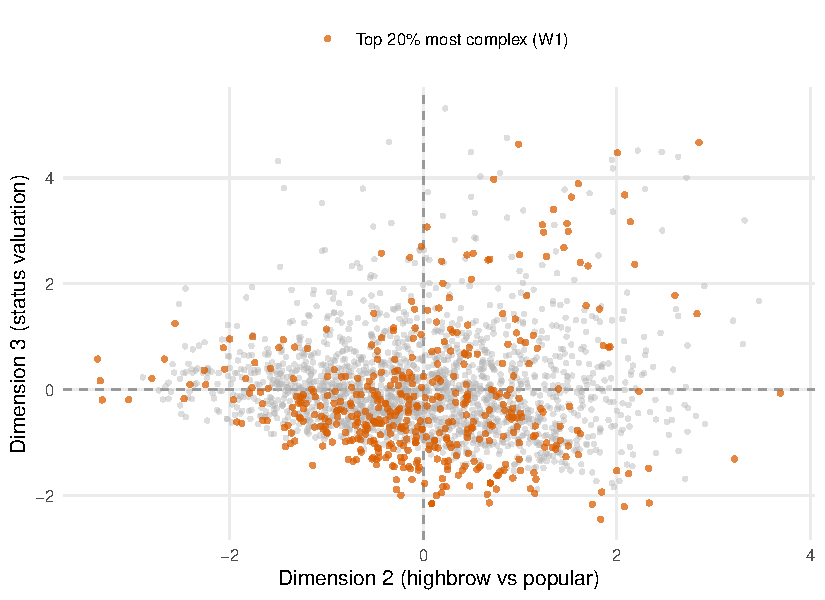
\includegraphics[width=.7\linewidth]{fig-antinomy-map} \caption{Individual factor map (dimensions 2--3). Grey points: all respondents; orange points: the 20\% of respondents with the highest complex-taste score on Dimension 1 ($W_1$).}
\label{fig:antinomy-map}
\end{figure}

The two measurement approaches also diverge in instructive ways (Table~\ref{tab:antinomy}). The geometric complex-taste score on Dimension 1 tracks the total number of complex tastes ($\rho = 0.31$; $\rho = 0.27$ with the total dispersion across the first three dimensions), but its counterparts on Dimensions 2 and 3 do not ($0.19$ and $-0.06$). The lesson is that geometric and combinatorial measures of complex tastes are related but not interchangeable: the dispersion of partial points captures \emph{how much} the aspects disagree overall, while the configuration counts capture \emph{which genres} the disagreement attaches to. They align where complex tastes are a matter of degree of engagement (Dimension 1) and diverge where they are a matter of hierarchical placement (Dimensions 2 and 3).

The configuration counts themselves have distinct geometric signatures, which is what makes them interpretable in the space. Distant praise sits squarely on the status-valuation dimension ($\rho = +0.79$, the pole anchored by the genre evaluations): it concentrates in consecrated genres whose fans' status respondents grant without liking or consuming them---the survey analogue of the unread bestseller. Guilty pleasures lean toward the popular pole of Dimension 2 ($\rho = -0.25$) and occupy the opposite, status-withholding pole of Dimension 3 ($\rho = -0.24$), with justified abstentions joining them there ($\rho = -0.33$). Taste poses are found among respondents high on the general-affirmation dimension ($\rho = 0.22$) who lean toward both the highbrow pole ($\rho = 0.34$) and the status-granting pole of Dimension 3 ($\rho = 0.37$).

\begin{table}[htbp]
\centering \caption{Spearman correlations between configuration counts (per respondent, out of 20 genres) and MFA coordinates and complex-taste scores ($N = 2{,}259$).}
\label{tab:antinomy}
\begin{tabular}{lcccccc}
\toprule
 & \multicolumn{3}{c}{MFA coordinates} & \multicolumn{3}{c}{Complex-taste scores} \\
\cmidrule(lr){2-4}\cmidrule(lr){5-7}
 & Dim 1 & Dim 2 & Dim 3 & $W_1$ & $W_2$ & $W_3$ \\
\midrule
Simple taste ($+++$) & 0.36 & 0.39 & 0.33 & $-$0.02 & 0.19 & 0.02 \\
Guilty pleasure ($++-$) & 0.69 & $-$0.25 & $-$0.24 & $-$0.03 & 0.16 & $-$0.21 \\
Pre-acquired taste ($-++$) & 0.10 & 0.10 & 0.16 & 0.10 & 0.06 & 0.04 \\
Taste pose ($+\,-+$) & 0.22 & 0.34 & 0.37 & $-$0.01 & 0.04 & 0.02 \\
Distanced consumption ($-+\,-$) & 0.05 & $-$0.11 & $-$0.03 & 0.13 & 0.01 & 0.02 \\
Justified abstention ($+\,--$) & 0.25 & 0.02 & $-$0.33 & $-$0.03 & 0.02 & $-$0.08 \\
Distant praise ($--+$) & $-$0.10 & 0.01 & 0.79 & $-$0.13 & $-$0.03 & $-$0.11 \\
Simple non-taste ($---$) & $-$0.84 & $-$0.11 & $-$0.19 & $-$0.31 & $-$0.25 & $-$0.01 \\
Total complex tastes & 0.74 & $-$0.01 & 0.09 & 0.31 & 0.19 & $-$0.06 \\
\bottomrule
\end{tabular}

\end{table}

\subsection{The Social Sources of Complex Tastes}
\label{sec:social}

To situate the sources of complex tastes socially, we project a set of respondent demographics---gender, race/ethnicity, age, education, parental education, household income, subjective social class, and census region---as supplementary variables onto the MFA representation. Supplementary variables do not influence the analysis: a category's coordinates are the barycenter of its members' positions in the common space, and the strength of each variable's association with each dimension is summarized by the correlation ratio $\eta^2$ (Tables~\ref{tab:eta} and \ref{tab:sup-coord}; Figure~\ref{fig:supplementary}).

\begin{table}[htbp]
\centering \caption{Correlation ratios ($\eta^2$) between supplementary demographic variables and the first three MFA dimensions.}
\label{tab:eta}
\begin{tabular}{lcccc}
\toprule
Variable & Dim 1 & Dim 2 & Dim 3 & Dim 4 \\
\midrule
Gender & 0.003 & 0.003 & 0.000 & 0.004 \\
Race/ethnicity & 0.026 & 0.048 & 0.004 & 0.255 \\
Age & 0.021 & 0.331 & 0.011 & 0.029 \\
Education & 0.016 & 0.053 & 0.000 & 0.003 \\
Parents' BA & 0.009 & 0.000 & 0.001 & 0.001 \\
Income & 0.000 & 0.016 & 0.003 & 0.002 \\
Subjective class & 0.001 & 0.055 & 0.005 & 0.012 \\
Census region & 0.004 & 0.005 & 0.003 & 0.016 \\
\bottomrule
\end{tabular}

\end{table}

\begin{table}[htbp]
\centering \caption{Supplementary category coordinates on the first three MFA dimensions (barycenters; $n$ = category size).}
\label{tab:sup-coord}
\begin{tabular}{llccccc}
\toprule
Variable & Category & $n$ & Dim 1 & Dim 2 & Dim 3 & Dim 4 \\
\midrule
Gender & Male & 1086 & -0.07 & 0.06 & 0.01 & -0.05 \\
Gender & Female & 1172 & 0.06 & -0.05 & -0.01 & 0.05 \\
\addlinespace
Race/ethnicity & Asian & 103 & -0.11 & 0.05 & 0.01 & 0.20 \\
Race/ethnicity & Black & 279 & 0.01 & -0.26 & -0.06 & 0.98 \\
Race/ethnicity & Hispanic & 364 & 0.32 & -0.42 & 0.13 & 0.34 \\
Race/ethnicity & White & 1448 & -0.10 & 0.16 & -0.02 & -0.30 \\
Race/ethnicity & >1 race & 53 & 0.77 & -0.28 & -0.12 & 0.33 \\
Race/ethnicity & Other & 11 & 0.40 & -0.02 & 0.14 & 0.17 \\
\addlinespace
Age & 18-29 & 477 & 0.22 & -0.74 & -0.09 & 0.13 \\
Age & 30-39 & 396 & 0.04 & -0.41 & 0.00 & 0.20 \\
Age & 40-49 & 429 & 0.12 & -0.18 & 0.17 & -0.11 \\
Age & 50-59 & 414 & -0.09 & 0.19 & 0.03 & -0.15 \\
Age & 60-69 & 296 & -0.21 & 0.71 & -0.00 & -0.19 \\
Age & 70+ & 246 & -0.31 & 1.23 & -0.18 & 0.11 \\
\addlinespace
Education & No diploma & 87 & -0.39 & -0.26 & 0.04 & 0.01 \\
Education & HS/GED & 468 & -0.24 & -0.25 & -0.01 & 0.04 \\
Education & Some college & 568 & 0.13 & -0.11 & -0.01 & 0.01 \\
Education & Associate & 221 & 0.12 & -0.09 & 0.00 & -0.08 \\
Education & BA & 621 & 0.05 & 0.09 & 0.02 & -0.02 \\
Education & MA & 215 & 0.06 & 0.51 & -0.04 & -0.04 \\
Education & Prof/PhD & 79 & 0.06 & 0.67 & -0.02 & 0.16 \\
\addlinespace
Parents' BA & Parents no BA & 1559 & -0.08 & 0.01 & 0.02 & -0.02 \\
Parents' BA & Parents BA & 700 & 0.17 & -0.03 & -0.05 & 0.04 \\
\addlinespace
Income & <\$25k & 911 & -0.01 & -0.16 & -0.01 & 0.03 \\
Income & \$25-49k & 526 & -0.01 & 0.04 & 0.03 & -0.05 \\
Income & \$50-74k & 477 & 0.03 & 0.12 & 0.07 & -0.03 \\
Income & \$75k+ & 345 & -0.01 & 0.19 & -0.11 & 0.02 \\
\addlinespace
Subjective class & Lower & 269 & -0.10 & -0.35 & -0.13 & 0.14 \\
Subjective class & Working & 832 & 0.02 & -0.23 & -0.03 & 0.04 \\
Subjective class & Middle & 1103 & -0.00 & 0.24 & 0.07 & -0.08 \\
Subjective class & Upper & 55 & 0.17 & 0.39 & -0.16 & 0.38 \\
\addlinespace
Census region & Northeast & 415 & 0.08 & -0.14 & 0.09 & 0.09 \\
Census region & Midwest & 502 & -0.12 & 0.07 & -0.03 & -0.14 \\
Census region & South & 812 & -0.01 & 0.00 & 0.01 & 0.11 \\
Census region & West & 529 & 0.07 & 0.04 & -0.06 & -0.10 \\
\bottomrule
\end{tabular}

\end{table}

\begin{figure}[htbp]
\centering
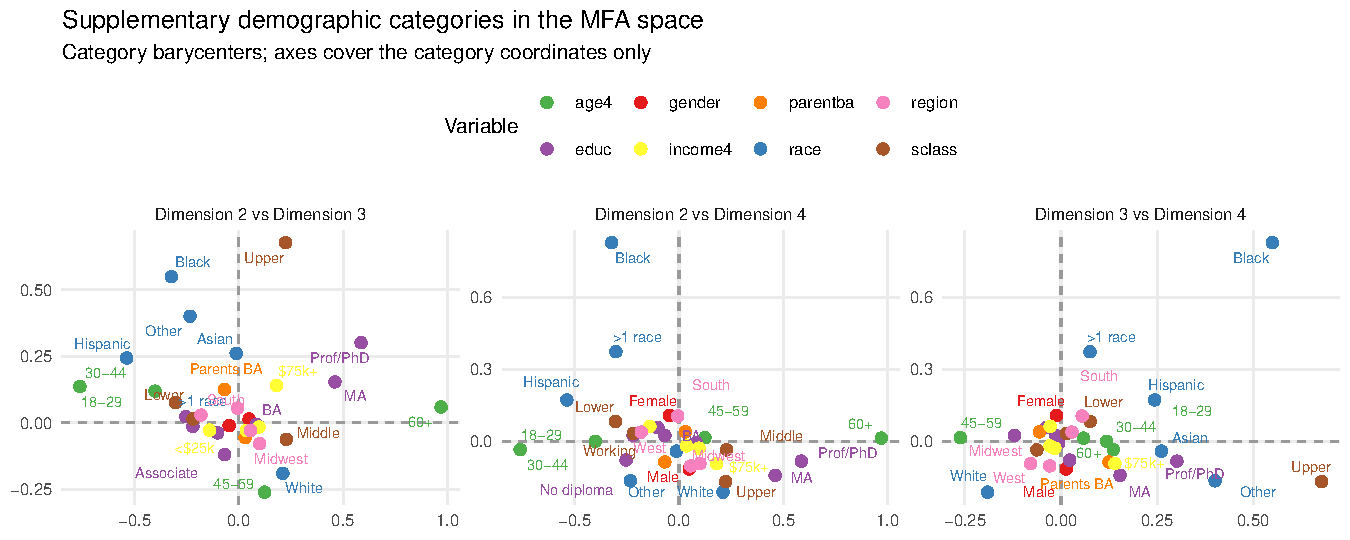
\includegraphics[width=\linewidth]{fig-supplementary} \caption{Supplementary demographic category barycenters (dimensions 2--3). Axis range covers the category coordinates only.}
\label{fig:supplementary}
\end{figure}

The social anatomy of the taste space runs primarily through the highbrow--popular dimension. Age is the strongest single anchor ($\eta^2 = 0.33$), with a nearly monotone gradient: respondents aged 18--29 sit at $-0.74$ on Dimension 2, those 30--39 at $-0.41$, those 40--49 at $-0.18$, those 50--59 at $+0.19$, those 60--69 at $+0.71$, and those 70 and older at $+1.23$---the genre hierarchy doubles as an age hierarchy. Education traces the same axis monotonically (No diploma $-0.26$, HS/GED $-0.25$, some college $-0.11$, Associate's degree $-0.09$, BA $+0.09$, MA $+0.51$, professional or doctoral degree $+0.67$; $\eta^2 = 0.05$), as does subjective social class (Lower $-0.35$, Working $-0.23$, Middle $+0.24$, Upper $+0.39$; $\eta^2 = 0.06$), with household income and race/ethnicity following more weakly (income from $-0.16$ to $+0.19$; Hispanic $-0.42$, Black $-0.26$, White $+0.16$). Gender and census region are negligible across all three dimensions.

The general-affirmation dimension is only weakly socially structured---no demographic variable exceeds $\eta^2 = 0.03$ on it---but the education pattern is instructive: the gradient is concentrated at the bottom of the credential distribution (No diploma $-0.39$, HS/GED $-0.24$) and flattens from some college upward ($+0.05$ to $+0.13$), indicating that generalized engagement with the genre system is most sharply differentiated at the entry into credentials rather than across their full range.

The status-valuation dimension, by contrast, is strikingly \emph{socially flat}. No demographic variable exceeds $\eta^2 = 0.011$ on it, and every category barycenter lies within about $\pm 0.2$ of the origin (Table~\ref{tab:sup-coord}). Whatever divides respondents on this dimension---the propensity to grant unambiguous high status to some genres' fans rather than others---is not captured by the standard stratification variables. This is consistent with the dimension's near-perfect geometric independence from the preference and consumption aspects established above, and it sharpens the interpretation of the status-valuation axis: it is not a credential or class gradient in disguise, but a structuring of taste whose social sources lie outside the standard demographic inventory.

\subsection{Who Has Complex Tastes?}
\label{sec:who}

The geometric measuring of complex tastes has one further advantage: $W_s(i)$ is a continuous, dimension-specific quantity, and can therefore serve directly as the outcome of a standard regression model---something the combinatorial count, a single coarse integer, does not allow. Table~\ref{tab:regression} reports OLS regressions of the three complex-taste scores on the same demographics projected as supplementary variables above. The headline result is the smallness of the associations: the full set of eight demographics accounts for $5.2\%$ of the variance in $W_1$, $2.0\%$ in $W_2$, and $2.1\%$ in $W_3$. Where respondents sit in the taste space is strongly socially patterned (Section~\ref{sec:social}); how much their aspects disagree is nearly socially unstructured. Complex tastes, on the geometric measure, are distributed across the social structure rather than concentrated within any of its segments.

The partial effects that do emerge are informative. Disagreement over engagement ($W_1$) is higher among respondents whose parents hold a BA ($+1.32$), among those who identify as more than one race ($+2.51$), and among those who identify as upper class ($+3.67$), and it declines with age ($-1.09$ at ages 30--39 through $-2.09$ at 70+, relative to the youngest cohort): aspect disagreement over liking, listening, and valuing is, if anything, concentrated among the advantaged rather than the excluded. Disagreement over the genre hierarchy ($W_2$) is nearly unpatterned: the only significant coefficient is a modestly higher score among the oldest cohort ($+0.63$). Disagreement over status valuation ($W_3$) is concentrated at the top of the class ladder ($+7.70$ for upper-class identifiers) and rises with age ($+2.04$ to $+2.73$ across the adult cohorts), with Hispanic respondents higher ($+1.89$) and those with an Associate's degree lower ($-3.79$) than their reference categories.

These findings are robust to a logarithmic transformation of the outcomes, which addresses the skew of the $W$ scores: the parental-education effect on $W_1$ persists (partial $F = 5.2$), as does the subjective-class effect ($F = 2.3$; the upper-class premium is $+0.40$ on the log scale), and a gender difference emerges on the log scale, with women showing lower $W_1$ ($F = 11.8$); the subjective-class effect on $W_3$ also persists ($F = 2.7$). The same demographics also predict the pairwise disagreement components of Dimension 3, with a consistent story: upper-class identification raises both preference--evaluation and consumption--evaluation disagreement (partial $F = 3.9$ and $4.9$), while preference--consumption disagreement is patterned primarily by parental education and subjective class ($F = 15.2$ and $9.3$). At the individual level, then, complex tastes are not the signature of any particular social location; they arise wherever the three weakly coupled measurement systems happen to diverge.

\begin{table}[htbp]
\centering \caption{OLS regressions of the geometric complex-taste scores on respondent demographics (unstandardized coefficients; standard errors in parentheses; $N = 2{,}259$). $^{***}p < 0.001$; $^{**}p < 0.01$; $^{*}p < 0.05$.}
\label{tab:regression}
\begin{tabular}{lccc}
\toprule
 & $W_1$ & $W_2$ & $W_3$ \\
\midrule
Gender (ref.~male) & & & \\
\quad Female & $-0.39$ (0.24) & $-0.06$ (0.13) & $0.38$ (0.22) \\
\addlinespace
Race/ethnicity (ref.~White) & & & \\
\quad Asian & $-0.15$ (0.58) & $-0.37$ (0.31) & $-1.50$ (0.53)$^{**}$ \\
\quad Black & $0.22$ (0.37) & $-0.16$ (0.20) & $0.15$ (0.34) \\
\quad Hispanic & $0.14$ (0.34) & $0.28$ (0.18) & $-0.13$ (0.31) \\
\quad >1 race & $2.04$ (0.77)$^{**}$ & $0.98$ (0.42)$^{*}$ & $1.94$ (0.71)$^{**}$ \\
\quad Other & $3.99$ (1.66)$^{*}$ & $-0.02$ (0.90) & $-1.57$ (1.52) \\
\addlinespace
Age (ref.~18--29) & & & \\
\quad 30--39 & $-0.79$ (0.38)$^{*}$ & $-0.52$ (0.21)$^{*}$ & $-0.16$ (0.35) \\
\quad 40--49 & $-0.64$ (0.37) & $-0.67$ (0.20)$^{***}$ & $0.15$ (0.34) \\
\quad 50--59 & $-1.14$ (0.38)$^{**}$ & $-1.01$ (0.21)$^{***}$ & $0.72$ (0.35)$^{*}$ \\
\quad 60--69 & $-1.22$ (0.43)$^{**}$ & $-0.98$ (0.23)$^{***}$ & $-0.04$ (0.39) \\
\quad 70+ & $-1.29$ (0.47)$^{**}$ & $0.08$ (0.25) & $-0.51$ (0.43) \\
\addlinespace
Education (ref.~no diploma) & & & \\
\quad HS/GED & $0.27$ (0.64) & $-0.44$ (0.35) & $-0.33$ (0.59) \\
\quad Some college & $0.55$ (0.64) & $0.01$ (0.34) & $0.22$ (0.58) \\
\quad Associate & $0.64$ (0.70) & $-0.07$ (0.38) & $-0.16$ (0.64) \\
\quad BA & $0.11$ (0.64) & $-0.13$ (0.35) & $-0.32$ (0.59) \\
\quad MA & $0.64$ (0.72) & $-0.18$ (0.39) & $-0.47$ (0.65) \\
\quad Prof/PhD & $0.16$ (0.88) & $0.04$ (0.47) & $1.25$ (0.80) \\
\addlinespace
Parents' BA (ref.~no BA) & & & \\
\quad Parents BA & $0.92$ (0.27)$^{***}$ & $-0.08$ (0.15) & $0.37$ (0.25) \\
\addlinespace
Household income (ref.~\$25k or less) & & & \\
\quad \$25--49k & $-0.41$ (0.32) & $-0.19$ (0.17) & $-0.07$ (0.29) \\
\quad \$50--74k & $0.08$ (0.34) & $-0.21$ (0.18) & $0.06$ (0.31) \\
\quad \$75k+ & $-0.26$ (0.40) & $-0.11$ (0.22) & $0.10$ (0.37) \\
\addlinespace
Subjective class (ref.~lower) & & & \\
\quad Working & $-0.06$ (0.40) & $-0.09$ (0.22) & $-0.16$ (0.37) \\
\quad Middle & $-0.20$ (0.42) & $0.07$ (0.23) & $0.26$ (0.38) \\
\quad Upper & $3.56$ (0.85)$^{***}$ & $0.22$ (0.46) & $-0.01$ (0.78) \\
\addlinespace
Census region (ref.~Northeast) & & & \\
\quad Midwest & $-0.38$ (0.37) & $-0.30$ (0.20) & $0.35$ (0.34) \\
\quad South & $-0.00$ (0.34) & $-0.33$ (0.18) & $-0.04$ (0.31) \\
\quad West & $0.24$ (0.36) & $-0.28$ (0.20) & $0.42$ (0.33) \\
\addlinespace
R$^2$ & 0.040 & 0.031 & 0.022 \\
$N$ & 2,259 & 2,259 & 2,259 \\
\bottomrule
\end{tabular}

\end{table}

\subsection{The Duality: Genres as Targets of Complex Tastes}
\label{sec:duality}

Complex tastes have a dual structure: individuals are \emph{sources} of complex tastes, and genres are \emph{targets}. To measure the target side, we transpose the analysis: individuals are now the twenty genres, and each aspect block contains one binary variable per respondent---whether that respondent likes, listens to, or grants unambiguous high status to the genre. Respondents whose answers are constant across all twenty genres within an aspect (who like nothing, listen to nothing, or are constant in their status attributions) define variables with an empty category; they contribute no genre discrimination and are dropped (83, 84, and 326 respondent-variables respectively). The transposition is not a mere rearrangement of the original solution. In simple correspondence analysis, the row and column clouds are dual, and the genre coordinates could be read off the original fit at no cost; but multiple correspondence analysis with a block structure breaks that duality. The category coordinates of the original analysis locate a genre through the composition of its audience---the barycenter of the respondents who affirm it---whereas the transposed analysis locates genres as objects, with distances computed over the respondent-indicators within each aspect block. Because MFA weights each block by the inverse of the first eigenvalue of its separate analysis, and transposing changes the separate analyses, the balancing weights and hence the eigen-decomposition differ: the transposed dimensions are optimized for the dispersion of the genre cloud rather than the respondent cloud ($\lambda_1 = 2.27$ here against $1.51$ above). And statistics defined over the individuals of an analysis---RV coefficients and partial points among them---do not survive transposition: the genre-level RV coefficients and the aspect-specific genre partial points reported below exist only in the transposed fit. The transposed MFA was implemented by direct application of the algorithm in \citet{pages2014mfa} and validated by reproducing the respondent-level \textsf{FactoMineR} solution: eigenvalues, global and partial coordinates, RV coefficients, and group contributions all agree to within $10^{-4}$.

\begin{figure}[htbp]
\centering
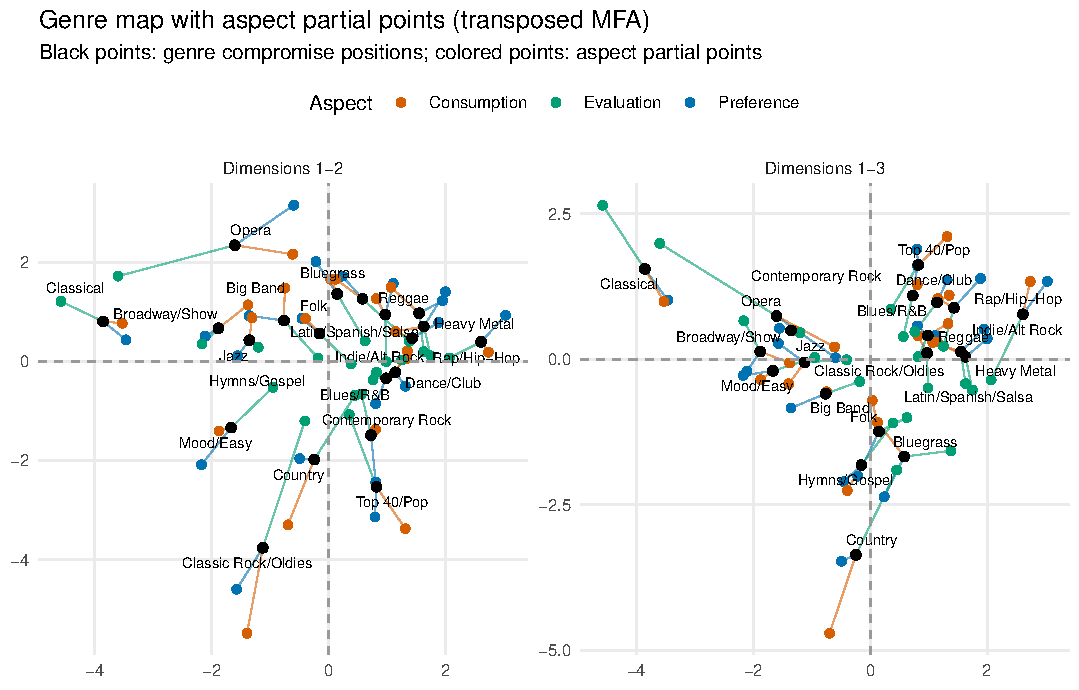
\includegraphics[width=\linewidth]{fig-genre-map} \caption{Genre map from the transposed MFA. Black points: genre compromise positions; colored points: aspect partial points (segments connect each genre's compromise to its aspect-specific positions).}
\label{fig:genre-map}
\end{figure}

The central result of the duality analysis is that, from the object side, the aspects \emph{agree}. The genre-level RV coefficients are $0.92$ (preference--consumption), $0.53$ (preference--evaluation), and $0.49$ (consumption--evaluation)---against $0.32$, $0.01$, and $0.01$ at the individual level. The disagreement that constitutes complex tastes is therefore not a property of the objects: the population that likes a genre, the population that listens to it, and the population that credits its fans with high status overlap substantially---far more than the corresponding individual-level profiles coincide. What varies---and what generates complex tastes---is whether a given individual occupies all three positions with respect to a given genre at the same time. Aspect independence is an individual-level achievement, not a genre-level partition.

\begin{table}[htbp]
\centering \caption{Genre target profiles: percentage of respondents holding each genre in each of Ma's configurations ($N = 2{,}259$).}
\label{tab:genre-profile}
\begin{tabular}{lcccccccc}
\toprule
 & \multicolumn{4}{c}{Complex configurations} & \multicolumn{4}{c}{Simple} \\
\cmidrule(lr){2-5}\cmidrule(lr){6-9}
Genre & Guilty & Pre-acq. & Pose & Dist. & Justif. & Distant & $+++$ & $---$ \\
\midrule
Classical & 9.9 & 1.1 & 13.5 & 1.5 & 12.4 & 19.5 & 19.3 & 22.8 \\
Opera & 2.4 & 0.8 & 7.3 & 0.9 & 5.8 & 39.5 & 4.3 & 38.7 \\
Jazz & 10.9 & 0.7 & 10.9 & 1.4 & 18.0 & 12.9 & 11.1 & 34.1 \\
Broadway/Show & 5.1 & 0.6 & 12.8 & 1.4 & 15.1 & 20.9 & 9.8 & 34.3 \\
Mood/Easy & 13.2 & 1.3 & 10.2 & 2.0 & 19.9 & 9.6 & 14.5 & 29.3 \\
Big Band & 6.2 & 0.3 & 9.8 & 0.9 & 17.8 & 12.8 & 5.3 & 47.0 \\
Classic Rock/Oldies & 23.8 & 0.8 & 8.2 & 2.2 & 19.5 & 3.9 & 21.6 & 20.1 \\
Country & 22.0 & 1.4 & 3.4 & 4.1 & 10.7 & 8.1 & 12.6 & 37.8 \\
Bluegrass & 4.9 & 0.1 & 4.4 & 0.9 & 17.2 & 8.5 & 2.2 & 61.7 \\
Folk & 4.2 & 0.5 & 6.4 & 0.8 & 13.7 & 11.3 & 3.9 & 59.2 \\
Hymns/Gospel & 9.5 & 0.8 & 6.6 & 1.2 & 12.6 & 13.4 & 9.6 & 46.4 \\
Latin/Spanish/Salsa & 9.4 & 0.7 & 4.7 & 1.3 & 9.2 & 14.0 & 5.7 & 55.0 \\
Rap/Hip-Hop & 15.8 & 1.2 & 1.4 & 4.6 & 6.9 & 8.8 & 7.0 & 54.3 \\
Blues/R\&B & 14.2 & 0.8 & 9.0 & 1.4 & 19.0 & 8.8 & 10.8 & 36.1 \\
Reggae & 7.7 & 0.4 & 5.2 & 1.3 & 15.7 & 9.6 & 4.0 & 56.3 \\
Top 40/Pop & 18.1 & 1.6 & 7.7 & 3.1 & 14.3 & 9.0 & 16.6 & 29.5 \\
Contemporary Rock & 12.5 & 1.0 & 8.9 & 2.3 & 18.7 & 10.0 & 10.9 & 35.7 \\
Indie/Alt Rock & 8.8 & 0.4 & 4.2 & 1.2 & 11.0 & 12.4 & 6.6 & 55.5 \\
Dance/Club & 11.3 & 1.0 & 8.5 & 1.5 & 15.9 & 14.1 & 7.4 & 40.4 \\
Heavy Metal & 9.8 & 0.3 & 2.1 & 1.3 & 8.5 & 10.9 & 4.4 & 62.6 \\
\bottomrule
\end{tabular}

\end{table}

The transposed space is itself strongly structured ($\lambda_1 = 2.27$, $14.6\%$ of the inertia; $\lambda_2 = 1.95$, $12.5\%$). Its second dimension is a \emph{configuration axis}: genres are ordered by the complex-taste profiles they attract (Table~\ref{tab:genre-profile}). At the positive pole sit the genres that respondents actively hold---in simple positive taste ($\rho = +0.77$), as taste poses ($+0.55$), as guilty pleasures ($+0.44$), or as justified abstentions ($+0.44$)---led by classic rock/oldies ($+3.7$), mood/easy listening ($+2.0$), country ($+1.8$), and top 40/pop ($+1.3$). At the negative pole sit the genres whose dominant relation is simple non-taste ($\rho = -0.73$): rap/hip-hop ($-1.7$), reggae ($-1.5$), Latin/Spanish/Salsa ($-1.3$), and heavy metal ($-1.3$)---together with opera ($-1.2$), whose relation to its audience is instead dominated by distant praise ($58.9\%$ of respondents hold it in that configuration). The duality is asymmetric in the way the theory of complex tastes anticipates: the prototypical guilty-pleasure genres are among the least credited with high status (evaluation rates of $8$--$14\%$ for classic rock/oldies, country, and top 40), and the prototypical distant-praise genre is the least consumed ($8.5\%$ for opera). The first dimension opposes genres whose typical relation is status without engagement---classical ($-3.6$), opera ($-3.0$), and Broadway/show tunes ($-2.1$), with distant-praise rates loading at $-0.82$ and taste-pose rates at $-0.58$---against genres held in guilty pleasure ($\rho = +0.75$) and distanced consumption ($+0.80$): top 40 ($+2.0$), rap/hip-hop ($+1.8$), classic rock/oldies ($+1.3$), and contemporary rock ($+1.3$)---well-known genres most often held with engaged disagreement.

Finally, the partial points locate where the aspects disagree about specific objects despite their global agreement. On the third dimension, the evaluation partial points of the consecrated genres are displaced toward positive values relative to their preference and consumption partial points (classical: $+2.3$ for evaluation against $+1.0$ for preference and $+0.9$ for consumption; opera: $+2.3$ against $-0.0$ and $+0.1$), while country shows the reverse displacement (evaluation $-0.8$ against $-3.1$ and $-4.1$). Status attributions, in other words, are distributed across genres in a way that only partially tracks who likes and who listens---echoing, at the level of the objects, the aspect independence established at the level of the sources.

\section{Discussion}

[DRAFT: The results establish three things. First, the three aspects of taste are empirically distinct structures, with evaluation nearly orthogonal to preference and consumption. Second, the shared space of taste is organized by a general-engagement gradient and a highbrow--popular hierarchy, both of which are visible in all aspects. Third, there exists a third-order dimension driven disproportionately by status evaluation---a candidate geometric locus for complex tastes. The operationalization of complex tastes is carried out in Section~\ref{sec:antinomies}, their social sources in Section~\ref{sec:social}, their individual-level correlates in Section~\ref{sec:who}, and the duality of sources and targets in Section~\ref{sec:duality}. The remaining steps are full introductory and discussion prose.]

\appendix

\section{The Combinatorial Measure: Ma's Eight Configurations}
\label{app:configurations}

The geometric measure locates complex tastes continuously in the common space. As a discrete complement, each genre--respondent pair can be classified into one of Ma's eight configurations from the binary triple of orientations (preference, consumption, evaluation): the simple taste $(+++)$, the simple non-taste $(---)$, and the six complex configurations.

Complex tastes are the statistical norm of this taste culture, not the exception. Figure~\ref{fig:configurations} reports the mean number of genres held in each configuration: the average respondent holds $10.2$ of the $20$ genres in a complex configuration, and only $12$ of $2{,}259$ respondents hold no complex configuration at all. The most frequent complex configuration is the \emph{justified abstention} ($3.3$ genres on average), followed by the \emph{guilty pleasure} ($3.2$) and \emph{distant praise} ($2.2$): respondents routinely like genres whose fans they do not credit with high status, grant high status to genres they neither like nor consume, and enjoy-and-consume genres whose fans they do not so credit. The taste pose ($1.0$) and the rare variants---distanced consumption ($0.4$) and the pre-acquired taste ($0.1$)---are comparatively infrequent, while the simple non-taste ($8.9$) is the single largest configuration.

\begin{figure}[htbp]
\centering
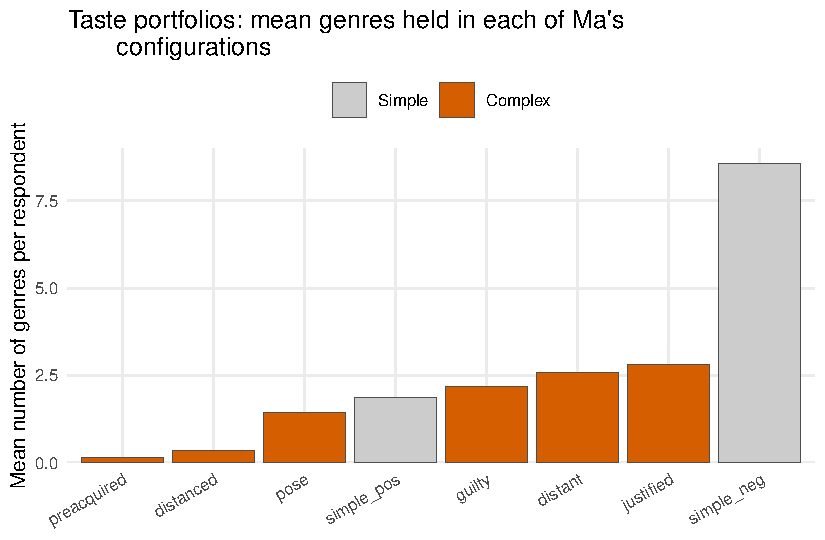
\includegraphics[width=.75\linewidth]{fig-configurations} \caption{Taste portfolios: mean number of genres held in each of Ma's eight configurations, per respondent. Orange: complex configurations; grey: simple ones.}
\label{fig:configurations}
\end{figure}

\bibliographystyle{plainnat}
\bibliography{references}

\end{document}
